\documentclass[12pt,a4paper]{article} %,fleqn
\usepackage{Diplo}
\usepackage[utf8]{inputenc} 
\usepackage[russian]{babel}

\usepackage[left=3cm,right=1.5cm,
top=2cm,bottom=2cm]{geometry}
\usepackage{longtable}
\usepackage{comment}
\usepackage{hyperref}
\usepackage[square, comma, sort&compress, numbers]{natbib}
\newtheorem{definition}{Определение}
\newtheorem{theorem}{Теорема}
\newtheorem{utv}{Утверждение}

\graphicspath{{../pics/}}

\begin{document}
	
\vskip 3mm

\setcounter{page}{1}
%%%%%%%% Титульный лист %%%%%%%%%%%%%%%%%%%%%%%%%%%%%%%%%
\begin{center}
	\thispagestyle{empty}
	
	{ Министерство науки и высшего образования Российской Федерации\\}

	
	
	{ Московский Физико-технический институт \\}
	
	{ (Государственный Университет) \\}
	
	{ Физтех-школа прикладной математики и информатики  \\}
	
	{ Кафедра технологий цифровой трансформации\\[4cm]}
	
	
	{ \bf \Large Выпускная квалификационная работа\\}
	
	{ \bf \Large{"Развитие инструментов предиктивной аналитики в целях повышения эффективности мониторинга проектов в сфере жилищного строительства"\\[1cm]} }
	
	{\bf {Студента 2-го курса Ефремова Сергея Владимировича}\\[3cm]}
	
\end{center}

\begin{flushright}
	\bf{Научный руководитель}\\
	\bf{кандидат экономических наук, доцент Помулев А. А.}\\[4cm]
\end{flushright}


\begin{center}
	Москва, 2022
\end{center}
%%%%%%%%%%%%%%%%%%%%%%%%%%%%%%%%%%%%%%%%%%%%%%%%%%%%%%%%%%%%%%%%

\newpage
\begin{abstract}

Рассматривается задача улучшения инструментов предиктивной аналитики, использующихся при мониторинге проектов в сфере жилищного строительства. Исследованы предложенные ранее схемы решения этой проблемы, на основе изученных материалов разработан подход по улучшению оценки вероятности просрочки выплаты займа застройщиком на основании отчетности, публикуемой в открытом доступе и уровне зависимости от импортируемых комплектующих и материалов. Предложен, реализован и протестирован алгоритм, основанный на алгоритмах нейросетевого обучения с использованием чисел Шепли.	

\end{abstract}

\newpage
\tableofcontents
 


\newpage
\section{Введение}


 

\newpage
\subsection{Цели и задачи работы}

\textbf{Цель и задачи исследования.} Целью исследования является построение модели предиктивной аналитики, которая позволит повысить эффективность процесса мониторинга проектов коммерческим банком в сфере жилищного строительства и улучшить качество прогнозирования вероятности просрочки платежа по сравнению с существующими моделями. Для реализации этой цели были поставлены следующие задачи:
\begin{itemize}
	\item изучить определение понятий: «мониторинг», «эффективность мониторинга», «предиктивная аналитика» для использования в настоящем исследовании;
	\item провести анализ существующих проектов и динамики их развития в сфере жилищного строительства;
	\item ознакомиться с текущим состоянием финансирования проектов в сфере жилищного строительства и нормативно-правовой базой;
	\item изучить процесс мониторинга проектов и методы их оценки коммерческим банком;
	\item исследовать типы моделей предиктивной аналитики и их применение в кредитном процессе;
	\item выделить основные проблемы процесса мониторинга проектов и определить возможности их решения с использованием инструментария предиктивной модели 
	\item разработать алгоритм внедрения разработанного инструментария в бизнес-процесс мониторинга
	\item рассчитать экономический эффект от внедрения модели 
\end{itemize}

\bigskip

\textbf{Научная новизна.} Используется нейросетевой подход к определению вероятности банкротства заемщика с выделением признаков, вносящих максимальный вклад с помощью, чисел Шепли. В работе предлагается коэффициент, позволяющий оценить зависимость застройщика от импортных комплектующих и материалов, а также уровень потенциального риска, обусловленного политическими ограничениями.

\bigskip

\textbf{Методы исследования.} Алгоритмы реализованы на языке программирования Python с использованием библиотек |||.

\bigskip

\textbf{Практическая ценность.} Полученная модель может быть использована в качестве встраиваемого модуля. Например, с её помощью можно:
\begin{itemize}
	\item корректировать оценку вероятности просрочки платежа застройщиком, учитывая его зависимость от импортируемых компонентов;
	\item дополнять существующие системы мониторинга объектов строительства показателем уровня зависимости от импортных компонентов и моделью оценки наиболее важных показателей, влияющих на просрочку.
\end{itemize}
%%%%%%%%%%%%%%%%%%%%%%%%%%%%%%%%%%%%%%%%%%%%%%%%%%%%%


\newpage
\section{Постановка задачи}


\subsection{Мониторинг проектов}\label{task}

изучить определение понятий: «мониторинг», «эффективность мониторинга», «предиктивная аналитика» для использования в настоящем исследовании

Мониторинг проекта - процесс измерения показателей выполнения проекта, сбора данных об исполнении проекта, информационного обслуживания управления проектом с целью выявления его соответствия желаемому результату и плану, с последующим представлением и распространением полученных данных.

Под контролем проекта понимается процесс сравнения фактических значений контрольных показателей с запланированными, последующего анализа отклонений, оценки тенденций и прогнозирования возможных альтернатив, разработки корректировок хода реализации проекта для улучшения прогноза.

Основными целями контроля и мониторинга инвестиционных проектов можно считать обеспечение:
\begin{itemize}
	\item своевременного достижения целей проекта с учетом согласованной стоимости;
	\item срочности, возвратности, платности и целевого использования предоставляемых банком кредитных ресурсов для финансирования проекта;
	\item своевременного информирования руководства банка о выявленных проблемах, прогнозирования рисков реализации проекта и разработка мер по их снижению;
	\item достижения заложенных в проекте показателей социально-экономической эффективности.  
\end{itemize}

Чаще всего при реализации проектов в сфере жилищного строительства выделяют следующие виды мониторинга:
\begin{itemize}
	\item мониторинг хода реализации инвестиционного проекта (сроков выполнения работ, бюджета проекта, расчетного времени окончания работ и расчетной стоимости проекта, организация технадзора и контрольных проверок);
	\item финансовый мониторинг (финансово-экономического состояния заемщика, исполнителя проекта, поручителей, гарантов, обеспечения по кредиту/кредитной линии; денежного потока, коэффициентов покрытия, целевого использования средств, исполнения заемщиком обязательств перед банком);
	\item мониторинг эффективности инвестиционного проекта (показателей, которые предусмотрены положением об экспертизе проектов банка).
\end{itemize}

Такое разделение обуславливается необходимостью не только контролировать текущую операционную деятельность, ведущуюся по проекту, исполнение финансовых обязательств участниками проекта и целевое использование средств, но и конечные результаты этой деятельности, которые выражаются в достижении целей проекта и достигнутой социально-экономической значимости.

Основными элементами систем мониторинга инвестиционных проектов являются:
\begin{itemize}
	\item финансовая, техническая и иная отчетность заемщика;
	\item экспертные оценки банковских специалистов по направлениям реализации проекта, независимые эксперты (технический надзор, финансовый аудит);
	\item календарно-сетевые графики работ, расчеты сроков ввода объекта в эксплуатацию и суммарной стоимости работ;
	\item данные автоматизированных информационных систем мониторинга инвестиционных проектов.
\end{itemize}

Последние и будут рассмотрены в первую очередь в данной работе.

Ключевые этапы мониторинга проектов:
\begin{itemize}
	\item этап подготовки проекта (начинается с момента одобрения займа/кредитной линии и заканчивается выделением финансовых средств);
	\item инвестиционная стадия проекта (непосредственное финансирование проекта);
	\item этап эксплуатации (следует до полного исполнения заемщиком платежных обязательств перед банком).
\end{itemize}

\subsection{Эффективность мониторинга}

Построением эффективных систем мониторинга занимались многие исследователи Д. Боуэр, Дж.Филлипс, Р.Фартел, Х.Керцнер[здесь будут ссылки на литературу]. Мониторинг в современных реалиях представляет из себя комплексную функцию проектного управления, в которую входит процедуры сбора, анализа и передачи информации о ходе реализации проекта, которая позволяет решить проблему своевременного принятия решений по проекту.

Основные задачи, которые решают системы мониторинга:
\begin{itemize}
	\item определение совокупности отслеживаемых индикаторов;
	\item организация обработки и агрегирования полученной информации;
	\item генерация текущей отчетности по проекту;
	\item интеграция функции мониторинга в информационную архитектуру предприятия, реализующего проект.
\end{itemize}

Принятие управленческих решений о формировании и развитии системы мониторинга проектов,о требуемом кадровом, техническом и финансовом обеспечении неизбежно связано с дополнительными затратами. Однако, потенциальные угрозы от финансирования убыточных или высокорисковых проектов также способны привести к значительным издержкам. Все это остро ставит вопрос о необходимости эффективного мониторинга проектов.

Основными подходами к изучению эффективности проектов являются:
\begin{itemize}
	\item целевой (предполагает анализ степени достижения целевых значений показателей);
	\item динамический (учитывает скорость изменения исследуемых показателей во времени и относительно друг друга);
	\item затратный (основан на сопоставлении затрат и результатов);
	\item ресурсный (исследует степень рациональности расходования ресурсов).
\end{itemize}

\subsection{Предиктивная аналитика}

Предиктивной аналитикой или продвинутой аналитикой называют ряд аналитических и статистических методов прогнозирования действий и поведения в будущем. В основе лежат статистические модели, позволяющие находить закономерности в исторических и транзакционных данных, что позволяет выделять потенциальные риски и возможности. Ключевые этапы составляющие процесс предиктивного анализа: подключение к данным, анализ и визуализация результатов исследований, развитие предложений и моделей данных, применение предиктивных моделей, оценка и прогнозирование будущих результатов.

В основе предиктивной аналитики лежит выявление связей между данными историческими и прогнозными результатами на их основе. Верхнеуровнево алгоритмы предиктивного анализа можно разделить на контролируемое и неконтролируемое обучение.

Контролируемое обучение принято разделять на две ключевые категории: регрессию для количественных ответов и классификацию для определения фактической принадлежности ответа к той или иной группе. 
 
Неконтролируемое обучение применяется для получения выводов из входных данных без разметки. Наиболее распространенный вид такого анализа - кластеризация, которую используют для поиска скрытых закономерностей в данных.

%%%%%%%%%%%%%%%%%%%%%%%%%%%%%%%%%%%%%%%%%%%%%%%%%%%%%

\newpage
\section{Обзор действующей практики}
\subsection{Анализ текущего состояния рынка жилищного строительства и тенденции развития}

В "Стратегии строительной отрасли до 2030 года" особое внимание уделяется наращиванию жилищного строительства, а также повышению комфортности жилищных условий. Так, в разделе "Целевые показатели по ипотеке и жилищному строительству" документа сформулирована задача увеличить обеспеченность населения жильем к 2024г. до $28-30~\text{м}^2$ на человека в среднем, а к 2030 году превысить этот уровень. Также предполагается повысить долю городов с благоприятной городской средой до 70\% к 2030г. Для того, чтобы достичь поставленных целей, необходимо нарастить объем жилищного строительства до не менее чем 120 млн.$~\text{м}^2$ в год (рис.~\ref{fig:develop_dynam}).

\begin{figure}[h]
	
	\centering
	
	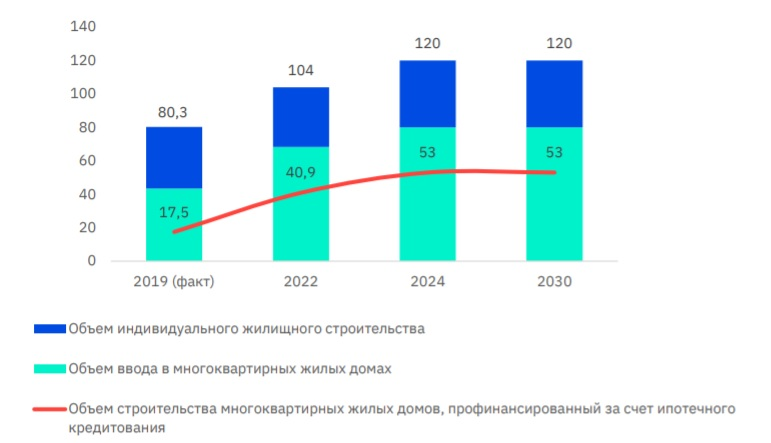
\includegraphics[width=0.7\linewidth]{develop_dynam.jpg}
	
	\caption{Классификация источников финансирования девелоперского проекта в зависимости от стадии его реализации.}
	
	\label{fig:develop_dynam}
	
\end{figure}

kdmcsjocndc 
Здесь должна быть динамика роста рынка строительства фактическая, сколько ввели, актуальность строек
Количество действующих кредитных договоров на конец 2021 года - 1 383

19\% приходится на Москву и Московскую область

Общая сумма действующих кредитных договоров - 6 247 550,0 млн. рублей

Рост за 2021 год на 113\% по количеству, и на 129\% по объему

В реестре проблемных застройщиков числятся – 650 организаций в 66 регионах РФ.



\subsubsection{Проект 1}


\subsubsection{Проект 2}

\subsection{Текущее состояние финансирования в сфере жилищного строительства}

\subsubsection{Основные источники финансирования }

В общемировой практике недвижимость считается одним из наименее рисковых направлений долгосрочного инвестирования с достаточно высоким уровнем рентабельности. Однако условия доступа, задающиеся высоким уровнем капитальным затрат, ограничивают круг потенциальных инвесторов. Так как крупные девелоперские проекты нуждаются в крупных капиталовложениях, реализация их за счет исключительно собственных средств для большинства компаний оказывается невозможной. Однако учитывая текущую практику, именно внешнее финансирование как нельзя лучше отражает суть девелопмента.
В зависимости от стадии реализации девелоперского проекта основные источники финансирования могут быть классифицированы в соответствии со схемой (рис.~\ref{fig:fin_source_clas}). 

\begin{figure}[h]
	
	\centering
	
	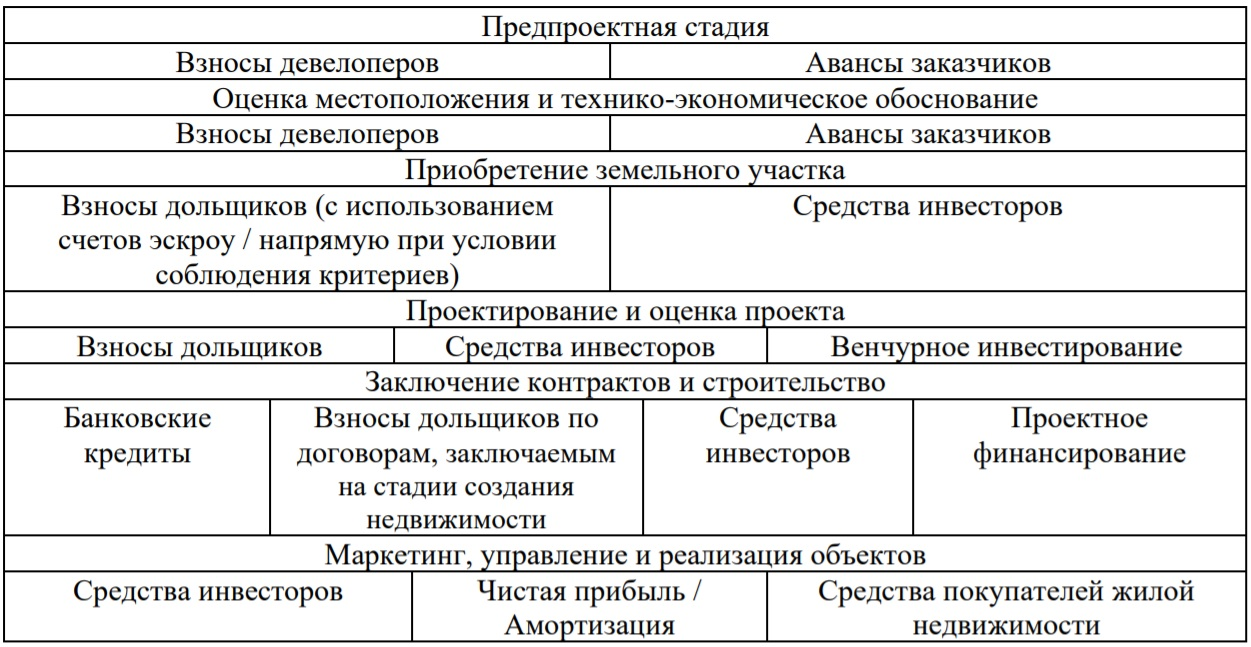
\includegraphics[width=0.7\linewidth]{fin_source_clas.jpg}
	
	\caption{Классификация источников финансирования девелоперского проекта в зависимости от стадии его реализации.}
	
	\label{fig:fin_source_clas}
	
\end{figure}

На первых этапах, как на самых рисковых, проект в основном финансируется за счет собственных средств. Далее, когда конфепция будущего объекта строительства уже разработана, привлекаются средства дольщиков. Финансирование проекта на стадии приобретения земельного участка носит рисковый характер, поэтому инвестиционные ресурсы оказываются самыми дорогими.

На этапе строительства используются банковские, облигационные займы и эскроу-счета. Этот этап проекта наиболее капиталоемкий  и требует значительных объемов инвестиционных ресурсов. На стадии продвижения привлечение заемных средств оказывается невозможным, так как займы выдаются под строительство.
В условиях Российского рынка задача усложняется высокими ценами на земельные участки, строительные материалы, значительными транспортными расходами и прочими издержками.

Наиболее распространенные механизмы рыночного финансирования девелоперских проектов в России:
\begin{itemize}
	\item договоры купли-продажи объектов жилой недвижимости;
	\item договоры участия в долевом строительстве;
	\item эскроу-счета.
\end{itemize}

До 2019 года наиболее распространенным механизмом финансирования было заключение договора участия в долевом строительстве (ДДС). Так на конец 2019 года в России было зарегистрировано 783 тысячи договоров ДДС. Такая популярность обусловлена рядом факторов[]: для покупателя - покупка на начальных этапах строительства позволяла сэкономить 25-35\% от стоимости готового объекта; использование инструментов снижения рисков, в частности государственная регистрация ДДС, страхование; в ряде случаев договоры предусматривали рассрочку платежей. Однако данный механизм имел ряд недостатков, в частности порожденная им проблема обманутых дольщиков. 
Для решения проблемы был разработан комплексный ряд мер, а именно были внесены правки в Федеральный закон от 30.12.2004г. №214-ФЗ "Об участии в долевом строительстве многоквартирных домов и иных объектов недвижимости и о
внесении изменений в некоторые законодательные акты Российской
Федерации". Как результат - с 1 июля 2019 года в России осуществляется переход на новую схему финансирования строительства многоквартирных домов через эскроу-счета.

\subsubsection{Эскроу-счета}

При применении данного подхода застройщик финансирует проект за счет собственных средств и банковских кредитов, а деньги дольщиков за проданные квартиры, хранящиеся на эскроу-счетах,  получает после сдачи проекта в эксплуатацию. 

По данным Банка России, уже на начало сентября 2020г. в банках было открыто почти 180 тыс счетов эскроу, на которых аккумулированно более 600 млрд. руб. При этом банки одобрили финансирование на 1,8 трлн руб., при общем объеме ссудной задолжности 667 млрд руб. По данным Банка России, средняя процентная ставка кредитной линии проектного финансирования составляла 4-6\% для договоров, заключенных до марта 2022 года. Средний срок рассмотрения заявки 30-45 дней. Особенность кредитования с применением счетов-эскроу заключается в том, что при значительном размере поступлений денежных средств участников долевого строительства на счета эскроу - ставка по кредиту снижается, в пределе она может быть снижена до 0.01\%.

\begin{figure}[h]
	
	\centering
	
	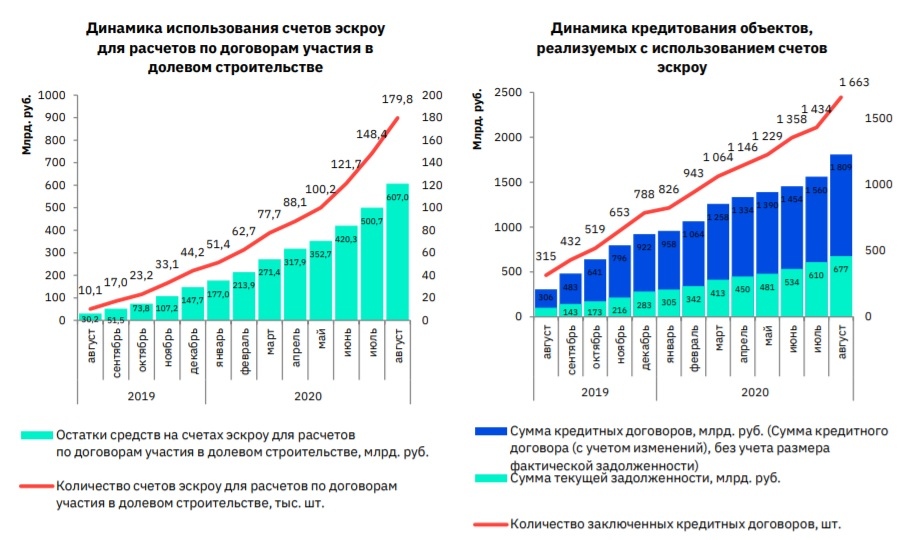
\includegraphics[width=0.7\linewidth]{eskrou_dynam.jpg}
	
	\caption{Динамика использования экроу счетов.}
	
	\label{fig:eskrou_dynam}
	
\end{figure}

Переход на новую модель финансирования жилищного строительства сопряжен с решением ряда систематических проблем. В первую очередь, данная модель предполагает замену средств дольщиков банковским кредитованием. Согласно расчетам ДОМ.РФ, для этого потребуется увеличение объемов кредитования застройщиков с 0,6 трлн руб. в 2018 г. до 6,4 трлн руб. в 2024 г. То есть на горизонте 4-5 лет, кредитный портфель застройщиков жилой недвижимости должен возрасти примерно в 10 раз(рис.~\ref{fig:eskrou_dynam}).

Обслуживание ссудной задолженности в рамках новой модели финансирования строительства жилой недвижимости возможно только при условии растущих объемов продаж квартир на первичном рынке. Основным драйвером спроса при этом считается развитие ИЖК и его льготных программ, субсидируемых государством. По итогам 2019 г. примерно 60\% квартир в новостройках и 50\% на вторичном рынке приобретены с помощью ИЖК.
Основными ограничителями спроса выступают повышение долговой нагрузки вследствие отставания динамики денежных доходов от платежей по кредиту и рост цен жилой недвижимости. Особенно остро обе эти проблемы ощутились на фоне повышения ключевой ставки ЦБ до 20\% в марте, ставки по ИЖК стали неподъемными даже по льготным программам ипотечного кредитования, а цены на недвижимость продолжили рост на фоне повысившихся инфляционных ожиданий национальной валюты.

Реформа отрасли строительства жилой недвижимости оставила девелоперов без возможности использовать бесплатные средства дольщиков. На начальных этапах перехода на проектное финансирование объем жилищного строительства в РФ снизился на 20 млн кв.м. Половина регионов Российской Федерации характеризуется нулевой или отрицательной маржинальностью жилищного строительства, обусловленной низкой платежеспособностью населения. Все это ограничивает застройщика при выборе источников финансирования. Также важен и тот факт, что кредит не покрывает все затраты проекта, а собственных средств застройщика может быть недостаточно для увеличения объема строительства. 

Для поддержания темпов роста, застройщики выходят на фондовый рынок. Доверие потенциальных инвесторов к ценным бумагам строительных компаний потенциально могут повысить структурирование девелоперских групп,  цифровизация компаний, повышение прозрачности их отчетности и формирование рейтинговой истории. Однако в связи со сложной политической обстановкой, правильно будет ориентироваться на привлечение  инвесторов внутри страны, так как доступ внешнего капитала весьма ограничен. Также исключительно важной становится и степень зависимости застройщика от внешнего капитала и импортных комплектующих, материалов и инструментов при строительстве. Чем выше степень зависимости, тем менее устойчивой становится девелопер и конкретные, финансируемые банком проекты, при оказании на них даже косвенного политико-экономического давления.

Все это приводит к необходимости постоянного проектного мониторинга и контроля потенциальных рисков со стороны банка, как у регулятора на новом сложившемся рынке жилищного строительства после введения счетов-эскроу.
  

\subsection{Процесс мониторинга проектов и методы оценки коммерческим банком}

Мониторинг коммерческим банком хода реализации проекта состоит из:
\begin{itemize}
	\item разработки календарно-сетевого графика создания объектов инвестиционного проекта и пояснения к нему;
	\item организации контроля за соблюдением плановых сроков, этапов, стоимостных параметров; назначением платежей; а также фактически выполненного объема работ и освоенных затрат на всех стадиях реализации проекта;
	\item выявления отклонений от плана реализации проекта и их последующего анализа, в том числе оценку влияния на сроки и бюджет проекта;
	\item разработки мер, направленных на снижение влияния отклонений, для выполнения проекта в запланированные сроки с установленным бюджетом;
	\item прогнозирования сроков окончания реализации проекта и суммарных затрат
	\item мониторинга исполнения дополнительных обязательств, в том числе организации и осуществления контроля над выполнением заемщиком, залогодателем и поручителями дополнительных условий и обязательств, установленных договором;
	\item организации экспертизы бюджетного проекта и проверки соответствия стоимостных параметров проекта текущему состоянию рынка строительных материалов, работ и оборудования;
	\item организации оперативного надзора за техническими и объемно стоимостными показателями проекта и анализа отчетной технической документации;
	\item отбора компаний для осуществления технического надзора;
	\item организации и проведении проверок объектов, находящихся на стадии строительства, в том числе проверок надзорных компаний;
	\item анализ отчетов строительных аудиторов и надзорных компаний;
	\item согласование видов рисков при страховании работ. 
\end{itemize}

Для проверки результатов реализации проекта также проводят мониторинг эффективности проекта. 
В ходе этого процесса выясняется достиг ли проект поставленных целей, особенно социально значимых и насколько он соответствует изначально заданным параметрам.
Мониторинг эффективности инвестиционного проекта состоит из:
\begin{itemize}
	\item мониторинга достижения запланированных конечных экономических показателей эффективности;
	\item мониторинг достижения запланированных конечных социально-экономических показателей эффективности для разных групп внешних потребителей результатов проекта;
	\item мониторинг эффективности инвестиций акционеров в капитал проектной кампании.
\end{itemize}

Резюмируя, мониторинг результатов развития инвестиционного проекта включает:
\begin{itemize}
	\item определение целевых показателей на предынвестиционной стадии;
	\item проведение оценки проектов в процессе их реализации на инвестиционной стадии.
\end{itemize}

При этом целевые показатели можно разделить на категории:
\begin{itemize}
	\item финансовые;
	\item экономические;
	\item экологические;
	\item показатели развития частного сектора.
\end{itemize}

Зачастую указанные выше показатели рассчитываются проектным офисом Банка вручную, для каждого проекта строится индивидуальная модель, сравниваются фактические данные и показатели план-графика и на основе отклонений делается прогноз по каждому объекту. Такой подход экспертной оценки имеет ряд преимуществ, таких как возможность рассмотреть каждый случай досконально и выделить все проблемные зоны. К сожалению, применение методики экспертных оценок является весьма время- и трудо- затратным процессом и невозможно при превышении определенной границы: числа объектов мониторинга в отношении на эксперта. Эта проблема вызвала необходимость разработки автоматизированных систем мониторинга проектов, которые могли бы по расчетным показателям и косвенным признакам подсветить наиболее проблемные объекты. Также стоит отметить, что наиболее эффективно не просто показывать объекты риска, но и индицировать по каким причинам объект считается проблемным. 

\subsection{Типы моделей предиктивной аналитики и их применение в кредитном процессе}

В основе применяемых в Банках систем мониторинга чаще всего лежат методы прямого сравнения с пороговыми показателями и прогнозными сравнениями или алгоритмы решающих деревьев. Причин у такого подхода несколько. В первую очередь, у Банка нет права на ошибку, поэтому система оценки проекта должна быть прозрачной и простой к оценке. Так у контролирующего ее работу эксперта будет возможность доступно интерпретировать результат автоматического расчета и оперативно сделать выводы о его корректности и необходимости корректировок оценки. Также сложные системы проектного мониторинга и  скоринговые-системы чаще всего требуют крупных вложений как на уровне разработки или закупки оценочных моделей, так и на этапе разворачивания решений на высокопроизводительных кластерах.

Среди наиболее популярных алгоритмов машинного обучения можно выделить методы представленные в~Таблице~\ref{Tab:1}.

\begin{center}
	\begin{longtable}{p{5cm}|p{10cm}}
		\hline Модель & Краткое описание    \\
		\endhead
		\hline Линейная множественная регрессия & Связывает зависимую переменную с линейной функцией независимых переменных. Задача сводится к поиску коэффициентов, при которых точность ответа, полученного в результате подстановки входных значений обучающей выборки в итоговую линейную функцию будет максимальна.  
		 \\
		 \hline
		Логическая регрессия & В основе лежит метод максимального правдоподобия. В целом, логика поиска весов аналогична  линейной регрессии, только оценивается вероятность принадлежности к одному из классов, решая задачу бинарной классификации.
		  \\
		  \hline
		Деревья классификации 
		 & Зависимость значения результирующей переменной представлена в виде иерархической ступенчатой структуры - дерева. 
		  \\
		  \hline
		 CHAID (Chi-squared Automatic Interaction Detection)& Критерий построения следующих узлов - значимость результата статистического теста. На каждом уровне дерева выявляется переменная оказывающая наибольшее влияние на результат. Также выделяется набор признаков, оказывающий максимальное влияние на результат.
		    \\
		\hline
		Нейронные сети&   
		 Каждый узел / нейрон - простой элемент, который можно промоделировать. Нейросеть позволяет обнаружить сложные и нелинейные зависимости между признаками и выходным результатом. Ключевая проблема - сложность интерпретации, структура нейросети не позволяет описать взаимосвязи в виде простой функции \\
		 \hline
		Случайный лес&
		Композиция решающих деревьев. Финальная классификация получается методом усреднения результата всех поддеревьев.
		\\
		\hline
		Метод опорных векторов&
		Ключевая идея метода заключается в повышении размерности пространства признаков, и поиске разделяющей гиперплоскости между исходными векторами значений
		\\
		\hline
		
		Байесовкий классификатор&Простой вероятностный классификатор, основанный на предположении о независимости признаков в исходном пространстве и последующем примении теоремы Байеса\\
		\\
		\hline 
		\caption{Наиболее распространенные алгоритмы машинного обучения в банковской сфере}
		\label{Tab:1}\\
	\end{longtable}

\end{center}

Большая часть представленных выше алгоритмов встречаются в кредитном скоринге. Задача мониторинга финансируемых проектов со стороны банка выглядит крайне близкой, разница заключается в том, что  клиент оценивается не только в момент одобрения кредитной линии, но и на протяжении всего жизненного цикла проекта. Основные направления кредитного скоринга:
\begin{itemize}
	\item Application-scoring или анализ заявок для определения потенциального риска выдачи кредита. Для задачи ПФ можем считать вероятность наличия просрочки у клиента;
	\item Fraud-scoring или скоринг против мошенничества, оцениваем вероятность того, что клиент является мошенником. Не актуально для задач ПФ;
	\item Behavioural-scoring или скоринг поведения заемщика. Для задачи ПФ, это вероятность что клиент передает несоответствующие действительности данные о ходе выполнения проекта;
	\item Collection-scoring определяет суровость мер, которые необходимо применить к заемщику, при просрочке.
\end{itemize}

Данная работа нацелена, в первую очередь на анализ адаптации Application скоринга для задач проектного финансирования.





%%%%%%%%%%%%%%%%%%%%%%%%%%%%%%%%%%%%%%%%%%%%%%%%%%%%%%

\newpage
\section{Формальная постановка задачи}

\subsection{Ключевые проблемы процесса мониторинга проектов}

\subsection{Возможности внедрения с учетом консервативности и систем безопасности банка}


%%%%%%%%%%%%%%%%%%%%%%%%%%%%%%%%%%%%%%%%%%%%%%%%%%%%%%

\newpage
\section{Описание модели}
 
\subsection{Этап предобработки данных}
 
\subsection{Ядро модели}

%%%%%%%%%%%%%%%%%%%%%%%%%%%%%%%%%%%%%%%%%%%%%%%%%%%%%

\newpage
\section{Результаты работы алгоритма}
\subsection{Пример полученных результатов - ключевые атрибуты}

\subsection{Сравнение результатов с другими методами}

\subsection{Сравнение результатов с оценкой предложенной метрики качества}


%%%%%%%%%%%%%%%%%%%%%%%%%%%%%%%%%%%%%%%%%%%%%%%%%%%%%

\newpage
\section{Экономический эффект от внедрения модели}

%%%%%%%%%%%%%%%%%%%%%%%%%%%%%%%%%%%%%%%%%%%%%%%%%%%%%


\newpage
\section{Заключение}



%%%%%%%%%%%%%%%%%%%%%%%%%%%%%%%%%%%%%%%%%%%%%%%%%%%%%


\newpage

\bibliographystyle{gost71s}
\bibliography{mylib}
\nocite{GV}

\end{document}